\subsection{Long-block Turbo autoencoder (TurboAE) AWGN check}
We additionally test a convolutional neural network (CNN) TurboAE-style encoder--decoder at block length \(64\), rate \(1/2\), and AWGN training point \(E_b/N_0=4\,\mathrm{dB}\).
The TurboAE models are trained through either analytic AWGN or the condition-wise Sinkhorn AWGN surrogate and then evaluated on analytic AWGN.
This complements the short-block multi-channel SER/BER study with a longer differentiable coding loop.

Fig.~\ref{fig:turboae-long-block-curve} shows the resulting BER and block error rate (BLER) curves over \(30\) seeds.
At the \(4\,\mathrm{dB}\) training point, analytic-channel training gives BER \(1.96\times 10^{-3}\) and BLER \(8.18\times 10^{-2}\), with 95\% confidence intervals (CIs) \(5.21\times 10^{-4}\) and \(2.30\times 10^{-2}\).
Training through the condition-wise Sinkhorn surrogate gives BER \(3.30\times 10^{-3}\) and BLER \(1.39\times 10^{-1}\), with 95\% CIs \(4.30\times 10^{-4}\) and \(1.91\times 10^{-2}\).
The surrogate preserves the waterfall trend, with a measurable gap to analytic-channel training.

\begin{figure}[!htbp]
\centering
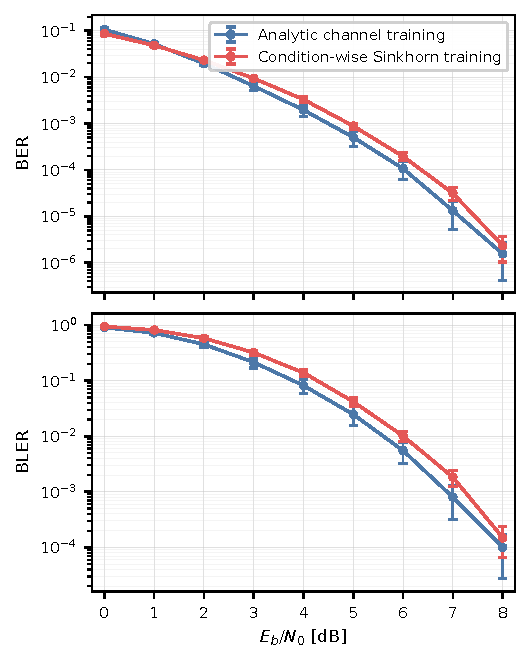
\includegraphics[width=0.84\columnwidth]{turboae_awgn_l64_ber_bler_curve_eval2k_column.pdf}
\caption{\textbf{Long-block TurboAE AWGN check.} CNN TurboAE models at block length \(64\), rate \(1/2\), are trained through analytic AWGN or the condition-wise Sinkhorn AWGN surrogate and evaluated on analytic AWGN over \(30\) seeds.}
\label{fig:turboae-long-block-curve}
\end{figure}
